\documentclass{article}
\usepackage[english]{babel}
\usepackage[utf8]{inputenc}
\usepackage{amsmath,amssymb}
\usepackage{parskip}
\usepackage{graphicx}
\usepackage{dsfont}
\usepackage{dsfont}
\usepackage{relsize}
\usepackage{array}
\newcommand{\bigsigma}{\makebox{\Huge\ensuremath{\sigma}}}
\newcommand{\bigpi}{\makebox{\Huge\ensuremath{\Pi}}}
\newcolumntype{C}[1]{>{\centering\let\newline\\\arraybackslash\hspace{0pt}}m{#1}}
\usepackage[top=2.5cm, left=3cm, right=3cm, bottom=4.0cm]{geometry}
\usepackage[table]{xcolor}
\usepackage[utf8]{inputenc}
\usepackage{textcomp}
\usepackage[utf8]{inputenc}
\usepackage{amsmath}
\usepackage{amssymb}
\usepackage{xcolor}
\usepackage{listings}
\usepackage{xstring}
\usepackage{graphicx}
\usepackage[export]{adjustbox}

\definecolor{dkgreen}{rgb}{0,0.6,0}
\definecolor{ltgray}{rgb}{0.5,0.5,0.5}

\makeatletter
\newif\ifcolname
\colnamefalse

\def\keywordcheck{%
\IfStrEq*{\the\lst@token}{select}{\global\colnametrue}{}%
\IfStrEq*{\the\lst@token}{where}{\global\colnametrue}{}%
\IfStrEq*{\the\lst@token}{from}{\global\colnamefalse}{}%
\color{blue}%
}
\def\setidcolor{%
\ifcolname\color{purple}\else\color{black}\fi%
}
\makeatother

\lstset{%
    backgroundcolor=\color{white},
    basicstyle=\footnotesize,
    breakatwhitespace=false,
    breaklines=true,
    captionpos=b,
    commentstyle=\color{dkgreen},
    deletekeywords={...},
    escapeinside={\%*}{*)},
    extendedchars=true,
    frame=single,
    keepspaces=true,
    language=SQL,
    otherkeywords={is},
    morekeywords={*,modify,MODIFY,...},
    keywordstyle=\keywordcheck,
    identifierstyle=\setidcolor,
    numbers=left,
    numbersep=15pt,
    numberstyle=\tiny,
    rulecolor=\color{ltgray},
    showspaces=false,
    showstringspaces=false, 
    showtabs=false,
    stepnumber=1,
    tabsize=4,
    title=\lstname
}

\newcommand{\tablespace}{\\[1.25mm]}
\newcommand\Tstrut{\rule{0pt}{2.6ex}}         % = `top' strut
\newcommand\tstrut{\rule{0pt}{2.0ex}}         % = `top' strut
\newcommand\Bstrut{\rule[-0.9ex]{0pt}{0pt}}   % = `bottom' strut
\title{Assignment-1 CS303}
\author{Shashank P \\ 200010048}
\date{\today}

\begin{document}
\maketitle




\section{Problem 1}
First we login as the root user. Then create a new username and passowrd.
We can assign previlages to the new user and login as that user.
\begin{lstlisting}[language=sql]
  create user 'Shashank'@'localhost' identified by 'MyPassword@123';
  grant all privileges on lab3.* to 'Shashank'@'localhost';
  /* Logout and login as user Shashank */
  create database lab3;
  use lab3;
\end{lstlisting}
\begin{figure}[!ht]
  \begin{center}
  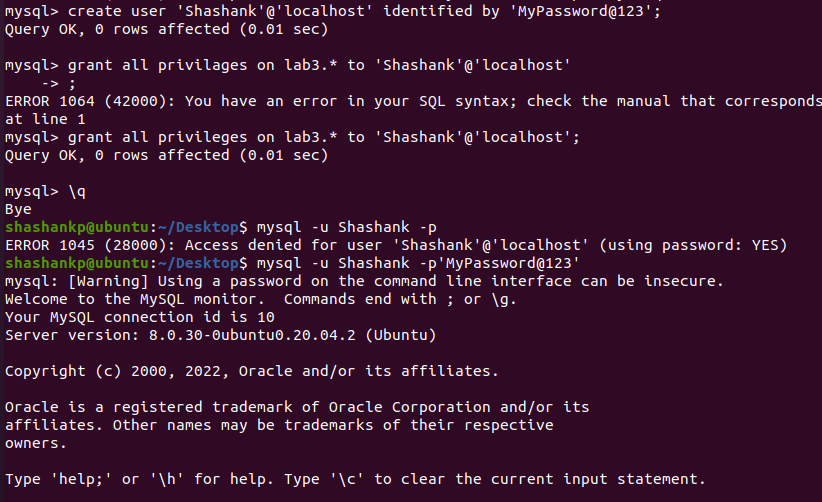
\includegraphics[scale=0.8]{new_user_1.png}
  \caption{Creation of User and adding previleges}
  \end{center}
\end{figure}


\section{Problem 2}
Based on the given information, we can come up with the following schema for the tables.
\begin{table}[ht]
  \centering
  \begin{center}
  \begin{tabular}{||C{3cm}||C{3cm}||C{3cm}||}
  \hline  
  \hline
  \textbf{Table} & \textbf{Primary Key}  & \textbf{Foreign Key}\\
  \hline \hline

  part & part\_no  & -- \\
  \hline \hline

  supplier & supplier\_no  & -- \\
  \hline \hline

  shipment & shipment\_no  & part\_no ref. part supplier\_no ref. supplier \\
  \hline \hline

  \end{tabular}
\end{center}
\caption{Keys in the given Schema}
\end{table}
\begin{lstlisting}[language=sql]
create table part(
    part_no int,
    part_name varchar(50) not null,
    color varchar(10),
    weight numeric(10, 5) check(weight>0),
    primary key (part_no)
);
create table supplier(
    supplier_no int,
    sup_name varchar(80) not null,
    city varchar(25),
    bank varchar(25),
    primary key (supplier_no)
);
create table shipment(
    shipment_no int,
    part_no int,
    supplier_no int,
    date DATE,
    quantity int check(quantity>=0),
    price numeric(15, 5) check(price>=0),
    primary key (shipment_no),
    foreign key (part_no) references part(part_no),
    foreign key (supplier_no) references supplier(supplier_no)
);
\end{lstlisting}
\begin{figure}[!ht]
  \begin{center}
  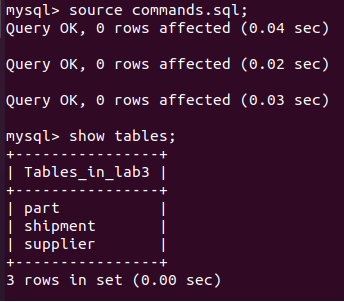
\includegraphics[scale=0.65]{add_tables.png}
  \caption{Adding relevant tables}
  \end{center}
\end{figure}


\section{Problem 3}
I have added one tuple to each table keeping in mind refrencial constraints.
\begin{lstlisting}[language=sql]
insert into part values(15, 'Rubber', 'red', '100');
insert into supplier values(10, 'John', 'Paris', 'Citi-Bank');
insert into shipment values(20, 15, 10, '2022-09-03', 50, 10);
\end{lstlisting}
\begin{figure}[!ht]
  \begin{center}
  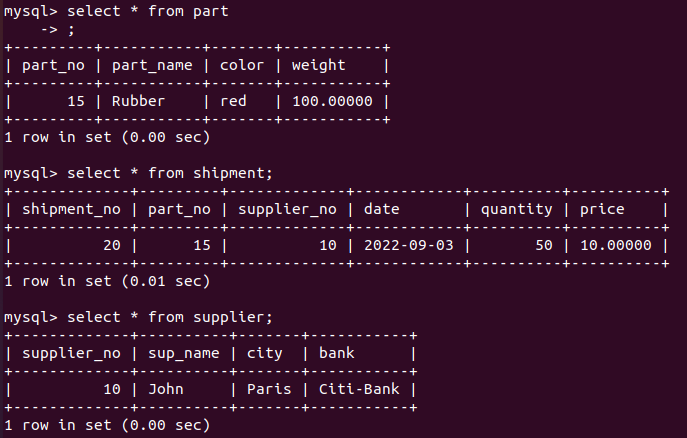
\includegraphics[scale=1]{added_one_tuple.png}
  \caption{Adding one tuple per table}
  \end{center}
\end{figure}

\newpage
\section{Problem 4}
Inserted multiple data points into each table. Referencial and Integrety constraints
were taken care of before inserting.
\begin{lstlisting}[language=sql]
insert into part values(30, 'Clip', 'yellow', '20');
insert into part values(45, 'Holder', 'red', '120');
insert into part values(60, 'Bolt', 'gray', '70');

insert into supplier values(25, 'Jane', 'Boston', 'American Bank');
insert into supplier values(40, 'Jack', 'New York', 'Western Union');

insert into shipment values(101, 15, 10, '2022-12-03', 18, 12.3);
insert into shipment values(102, 15, 25, '2020-03-04', 45, 15.6);
insert into shipment values(103, 15, 25, '2022-01-06', 150, 2.56);
insert into shipment values(104, 15, 40, '2020-05-12', 60, 24);

insert into shipment values(105, 30, 10, '2021-05-25', 100, 65);
insert into shipment values(106, 30, 40, '2022-04-16', 120, 12.35);
insert into shipment values(107, 30, 25, '2022-03-11', 50, 1.22);
insert into shipment values(108, 30, 10, '2021-02-28', 80, 90);

insert into shipment values(109, 45, 10, '2020-11-27', 95, 45.12);
insert into shipment values(110, 45, 10, '2022-10-14', 11, 120);
insert into shipment values(111, 45, 25, '2021-09-07', 154, 0.5);
insert into shipment values(112, 45, 25, '2022-09-01', 20, 1.3);

insert into shipment values(113, 60, 25, '2020-05-05', 8, 65);
insert into shipment values(114, 60, 40, '2021-06-04', 1, 1200);
insert into shipment values(115, 60, 40, '2021-08-21', 60, 100);
insert into shipment values(116, 60, 25, '2022-12-18', 90, 0.30);
\end{lstlisting}
\newpage
\begin{figure}[!ht]
  \begin{center}
  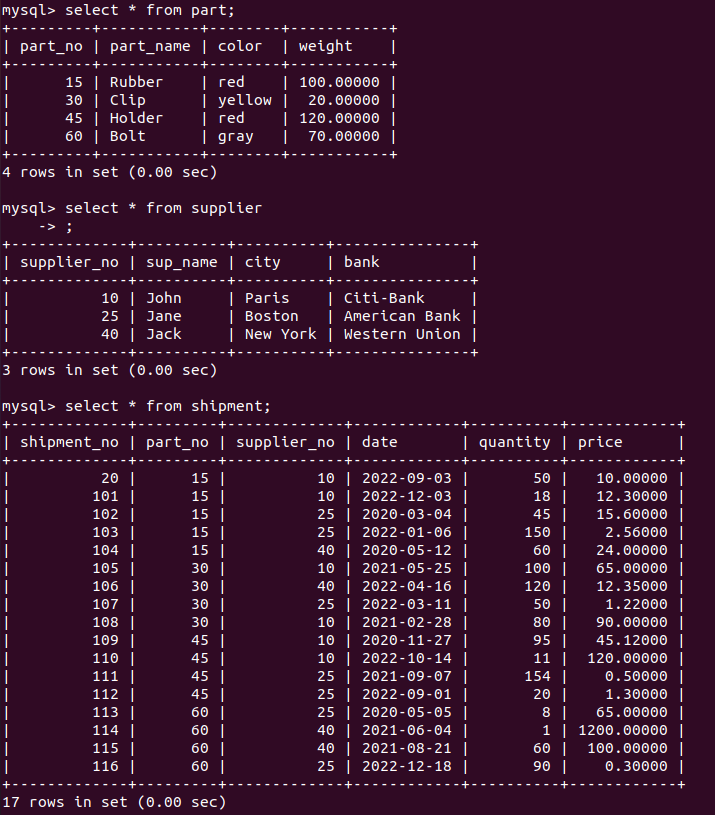
\includegraphics[scale=1]{added_multiple_data_4.png}
  \caption{Adding multiple rows to each table}
  \end{center}
\end{figure}
\newpage

\section{Problem 5}

\subsection{Part (i)}
Firstly we find the natural join of all 3 tables. From this we can select 
names and IDs of suppliers who have sold parts with colour red.
\begin{lstlisting}[language=sql]
select distinct supplier.supplier_no, supplier.sup_name
from (shipment natural join part) natural join supplier
where part.color='red';
\end{lstlisting}
\begin{figure}[!ht]
  \begin{center}
  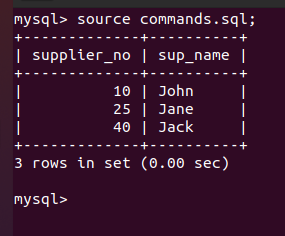
\includegraphics[scale=1]{red_supply.png}
  \caption{Suppliers who have supplied red parts}
  \end{center}
\end{figure}

\subsection{Part (ii)}
We can group the shipment table by \textit{supplier\_id}. We can use the
aggregate \textit{sum} function to get the total cost. Then to get the
the names of the suppliers, we perform a natural join with \textbf{supplier} table.
\begin{lstlisting}[language=sql]
select supplier.supplier_no, supplier.sup_name, supplier_costs.total_cost, supplier.bank
from supplier natural join (
        select shipment.supplier_no, sum(shipment.quantity * shipment.price)
        from shipment natural join supplier
        group by shipment.supplier_no
    ) 	as supplier_costs(supplier_no, total_cost);
\end{lstlisting}
\begin{figure}[!ht]
  \begin{center}
  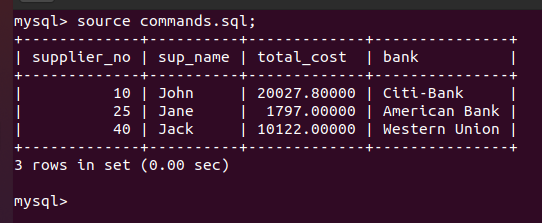
\includegraphics[scale=0.57]{cost_per_supplier.png}
  \caption{Total cost of each supplier}
  \end{center}
\end{figure}

\subsection{Part (iii)}
We can group the shipment table by \textit{supplier\_id}. We can use the
aggregate \textit{sum} function to get the total cost. Then to get the
the names of the suppliers, we perform a natural join with \textbf{supplier} table.
\begin{lstlisting}[language=sql]
with total_parts(value) as (select count(distinct part_no) from part), 
    sup_total(supplier_no, value) as (select supplier_no,count(distinct part_no) from shipment group by supplier_no)
select supplier.supplier_no, supplier.sup_name
from total_parts, (supplier natural join sup_total)
where total_parts.value=sup_total.value
\end{lstlisting}
\begin{figure}[!ht]
  \begin{center}
  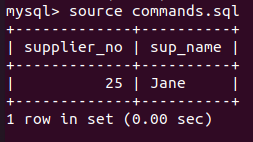
\includegraphics[scale=1]{5c.png}
  \caption{Supplier who supplied all parts}
  \end{center}
\end{figure}

\end{document}
